\documentclass[10pt]{article}
\usepackage{icmlko}

\icmlmeta{IP 파운데이션 월드모델}{248}{큰 수와 큰 효과}{노트 247이 제일 크다고 짚은 $+$0.131 은 잡음이었다 --- 그런데 잡음을 걷으니 상쇄가 네 배에서 열아홉 배로 뚜렷해진다}

\begin{document}

\twocolumn[
\icmlheader

\begin{abstract}
노트 247은 부호화 규약 하나(도메인 안 백분위)가 판을 $-$0.0036 밖에 안
움직이는데 아이돌을 \textbf{$+$0.131} 움직인다고 보고하며 그것을 제일 큰
자리바꿈으로 짚었다. \textbf{그 수는 SE 없이 읽은 수다.} 도메인마다 $\rho$
를 붓스트랩해 보니 SE 가 웹툰 0.034(711건)에서 아이돌 \textbf{0.207}
(25건)까지 \textbf{여섯 배} 벌어져 있다. 아이돌의 짝 SE 는 0.212 라
$t{=}0.62$ --- 잡음이다. 게다가 아이돌은 \textbf{짝 SE 가 주변 SE 보다
큰 유일한 도메인}이다(0.212 대 0.207). 짝짓기가 도움이 안 된다는 것은 두
예측이 거의 무상관이라는 뜻이고, 나머지 여덟에서는 짝 SE 가 주변의
3분의 1 이하다(웹툰 0.0095 대 0.0337). \textbf{그런데 잡음을 걷으니 노트
247의 결론이 약해지는 게 아니라 강해진다.} $|t| \ge 2$ 인 둘만 남기면 ---
웹툰 $+$0.024($t{=}2.49$) · 게임 $-$0.084($t{=}-2.31$) --- 총량 0.0136에
순 $-$0.0007 로 \textbf{상쇄가 4배가 아니라 19배}다. 잡음은 상쇄되지 않고
양쪽에 흩어져 있었으므로, 그것을 빼면 남는 것은 순수한 자리바꿈이다.
\texttt{rank.spread} 를 고쳐 짝 SE 와 ``진짜 총량''을 같이 들고 다니게
했다. 이제 그 함수는 제일 큰 도메인으로 아이돌이 아니라 \textbf{게임}을
가리킨다.
\end{abstract}
]

\section{내가 짚은 수를 안 재고 있었다}

노트 247은 도메인별 $\rho$ 변화를 아홉 줄로 적고 제일 큰 것을 굵게 했다 ---
아이돌 $+$0.131. 그 줄에 SE 가 없었다. 아이돌은 유보가 \textbf{25건}이다.

도메인마다 유보 표본을 2,000번 되뽑아 $\rho$ 의 SE 와, 두 판을 같은 되뽑기로
견준 \emph{짝} SE 를 같이 냈다.

\begin{center}\small
\begin{tabular}{lrrrrr}
\hline
도메인 & $n$ & SE & 차 & 짝 SE & $t$ \\
\hline
웹툰 & 711 & 0.034 & $+$0.024 & 0.0095 & $\mathbf{+2.49}$ \\
게임 & 223 & 0.049 & $-$0.084 & 0.0364 & $\mathbf{-2.31}$ \\
모바일 & 441 & 0.035 & $-$0.011 & 0.0086 & $-$1.32 \\
애니 & 606 & 0.034 & $-$0.011 & 0.0093 & $-$1.18 \\
\textbf{아이돌} & \textbf{25} & \textbf{0.207} & $\mathbf{+0.131}$ &
  \textbf{0.2116} & $\mathbf{+0.62}$ \\
도서 & 163 & 0.073 & $-$0.025 & 0.0431 & $-$0.58 \\
세계애니 & 300 & 0.045 & $+$0.004 & 0.0077 & $+$0.51 \\
팝업 & 59 & 0.113 & $-$0.005 & 0.0344 & $-$0.14 \\
펀딩 & 80 & 0.112 & $+$0.006 & 0.0461 & $+$0.13 \\
\hline
\end{tabular}
\end{center}

\begin{figure}[t]
\centering
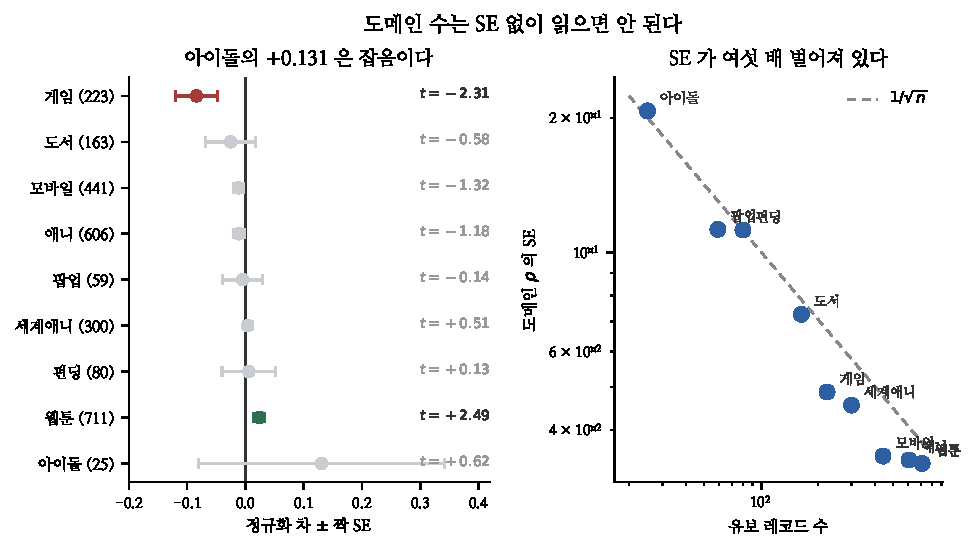
\includegraphics[width=\columnwidth]{figs/se.pdf}
\caption{왼쪽 --- 차와 짝 SE. 회색은 $|t| < 2$ 다. 오른쪽 --- 표본 수와 SE,
점선이 $1/\sqrt{n}$.}
\end{figure}

\textbf{제일 큰 수가 제일 작은 효과였다.} 아이돌 $+$0.131 은 $t{=}0.62$ 이고,
그것보다 다섯 배 작은 웹툰 $+$0.024 가 $t{=}2.49$ 다.

\section{짝짓기가 안 듣는 도메인}

표에 한 줄 더 읽을 것이 있다. 짝 SE 는 보통 주변 SE 보다 훨씬 작다 --- 같은
레코드를 두 판에서 함께 뽑으므로 공통 잡음이 지워지기 때문이다. 웹툰은
0.0337 $\to$ 0.0095 로 3분의 1 이하고, 세계애니는 0.045 $\to$ 0.0077 로
6분의 1 이다.

아이돌만 반대다 --- 0.207 $\to$ \textbf{0.2116}. \textbf{짝짓기가 도움이 안
된다.} 두 판의 예측이 거의 무상관이라는 뜻이고, 25건에서 열일곱 축이
백분위로 다시 매겨지면 순위가 통째로 다시 그려진다는 말이다. 노트 247이
``25건인데 규약에 0.131 흔들린다''고 이상해한 것의 답이 여기 있다 ---
\textbf{흔들린 게 아니라 애초에 잡고 있는 게 없었다.}

\section{잡음을 걷으니 결론이 강해진다}

\begin{figure}[t]
\centering
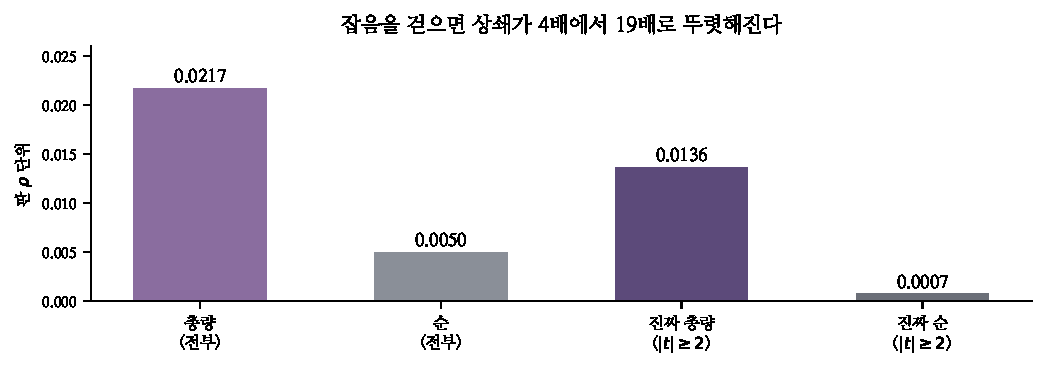
\includegraphics[width=\columnwidth]{figs/cancel.pdf}
\caption{$|t| \ge 2$ 인 둘만 남기면 총량은 63\%로 줄지만 순은 7분의 1 로
줄어, 상쇄비가 커진다.}
\end{figure}

보통 이런 정정은 원래 주장을 약하게 만든다. 여기서는 반대다.

\begin{center}\small
\begin{tabular}{lrrr}
\hline
 & 총량 & 순 & 상쇄 \\
\hline
아홉 전부 & 0.0217 & $-$0.0050 & 4배 \\
$|t| \ge 2$ 인 둘 & 0.0136 & $-$0.0007 & \textbf{19배} \\
\hline
\end{tabular}
\end{center}

까닭은 단순하다. 잡음 일곱은 부호가 제멋대로라 \emph{순}에 $-$0.0043 을
보태고 있었다 --- 진짜 상쇄를 가리는 잡음이었다. 그것을 빼면 남는 것은
웹툰 $+$0.024 와 게임 $-$0.084 뿐이고, 무게를 실으면 $+$0.0065 와
$-$0.0072 로 \textbf{거의 정확히 맞부딪친다.}

노트 247의 결론 --- ``판 $\rho$ 는 이 결정에 대해 잘못된 자다'' --- 은 그대로
서 있고, 오히려 더 깨끗한 형태로 선다. \textbf{큰 도메인 하나가 얻고 다른
하나가 그만큼 내놓는데, 판은 아무 일도 없었다고 보고한다.}

\section{함수를 고쳤다}

\texttt{rank.spread} 가 짝 SE 와 $t$ 를 같이 내고, ``진짜 총량''($|t| \ge 2$
만)을 따로 들고 다니게 했다. 제일 큰 도메인도 \emph{유의한 것 중에서} 고른다.

\begin{center}\small
\begin{verbatim}
{"순": -0.005, "총량": 0.0217,
 "진짜 총량": 0.0136, "진짜 순": -0.0007,
 "상쇄배": 18.8, "제일 큰 도메인": "게임",
 "제일 큰 값": -0.084, "진짜 몇": 2}
\end{verbatim}
\end{center}

노트 247이 쓴 그대로 돌리면 이제 아이돌이 아니라 \textbf{게임}이 나온다.

\section{되돌아보면}

이 실험실에는 표본 수를 함께 보라는 규약이 이미 있었다. 노트 132는 팝업
학습이 열여섯 행이라 자기 계수가 잡음이라고 적었고, F21은 그래서
\texttt{min\_rows=150} 을 둔다. 노트 231은 판정치가 죽은 도메인을 숨긴다고
적고 덮음을 판정치에 붙였다.

그런데 \textbf{도메인별 $\rho$ 를 보고할 때는 그 규약을 안 지키고 있었다.}
노트 224의 \texttt{by\_kind}, 노트 231의 \texttt{coverage}, 노트 247의
\texttt{spread} 가 다 도메인별 수를 내는데 셋 다 SE 가 없다. 이번에 고친
것은 셋 중 하나다.

\paragraph{남은 것}
\begin{center}\small
\begin{tabular}{ll}
\hline
갈래 & 왜 \\
\hline
\texttt{by\_kind} & 선호형/양형 몫도 SE 없이 보고한다 \\
아이돌 · 팝업 & SE 0.11$\sim$0.21. 이 둘로는 아무것도 못 정한다 \\
게임 $-$0.084 & 정규화로 제일 많이 잃는 진짜 효과. 왜인가 \\
25건 도메인 & 판에 남겨 두는 게 맞나 --- 몫 1.0\%에 SE 0.21 \\
\hline
\end{tabular}
\end{center}

\paragraph{규약} \textbf{도메인별 수는 SE 와 함께 적는다.} 유보 200건 아래
도메인(아이돌 25 · 팝업 59 · 펀딩 80 · 도서 163)의 수는 $\pm$0.07 $\sim$
$\pm$0.21 이라, 소수 둘째 자리를 근거로 쓰면 안 된다.

\end{document}
